\documentclass[13pt, a4paper, twoside]{mwart}
\usepackage[a4paper]{geometry}
\geometry{left=3cm}
\geometry{right=1.5cm}
\geometry{top=2cm}
\geometry{bottom=1.5cm}
\usepackage[pdftex]{graphicx}
\graphicspath{{img/}}

\usepackage[utf8]{inputenc}
\usepackage{polski}
\usepackage[polish]{babel}
\usepackage{tabularx}
\usepackage{datetime}
\usepackage{listings}
\lstset{basicstyle=\footnotesize}

\newcommand{\coursename}{Modelowanie i Analiza Systemów}
\newcommand{\labnumber}{2}
\newcommand{\labname}{Testbench układu decymacyjnego}
\newcommand{\studentname}{Maciej Stanek}
\newcommand{\studentnumber}{122352}
\newdate{labdate}{16}{3}{2018}
\newdate{labreportdate}{30}{3}{2018}

\usepackage{fancyhdr}
\pagestyle{fancy}
\fancyhead[RO,LE]{\thepage}
\fancyhead[LO]{\textbf{LAB\#\labnumber} \labname}
\fancyhead[RE]{\coursename}
\fancyfoot{}

\usepackage{xcolor}
\usepackage{framed}
\colorlet{shadecolor}{gray!10}
\newcounter{taskcounter}
\newcommand{\task}[1]{
  \stepcounter{taskcounter}
  \vspace{0.2cm}
  \begin{shaded}
    \noindent\textbf{Zadanie \thetaskcounter:} \textit{#1}%
  \end{shaded}
  \vspace{0.2cm}}

\renewcommand{\labelitemi}{$\bullet$}

\begin{document}

\begin{center}
  \textbf{\LARGE{Sprawozdanie z laboratorium}}
\end{center}

\noindent
\begin{tabularx}{\linewidth}{rX}
  \textbf{Przedmiot} & \coursename \\
  \textbf{Temat laboratorium} & \labname \\
  \textbf{Numer laboratorium} & \labnumber \\
  \textbf{Imię i nazwisko} & \studentname \\
  \textbf{Numer indeksu} & \studentnumber \\
  \textbf{Data wykonania} & \displaydate{labdate} \\
  \textbf{Data sprawozdania} & \displaydate{labreportdate} \\
\end{tabularx}

\vspace{0.3cm}
\noindent\hrulefill

%%%%%%%%%%%%%%%%%%%%%%%%%%%%%%%%%%%%%%%%%%%%%%%%%%%%%%%%%%%%%%%%%%%%%%%%%%%%%%%

\task{Opis koncepcji układu decymacyjnego i wyjaśnienie jego działania.}

Układ decymacyjny to urządzenie zliczające ilość zer i jedynek w kolejnych segmentach ciągu bitowego o stałej szerokości OSR. Licznik rozpoczyna zliczanie na wartości OSR i inkrementuje bądź dekrementuje jego wartość po otrzymaniu wartości odpowiednio 1 lub 0. Po analizie OSR bitów, układ wystawia na wyjściu wyznaczoną wartość końcową (w przedziale od 0 do 2OSR), resetuje się do wartości OSR i rozpoczyna kolejny cykl.

\task{Opis koncepcji działania całego układu testbenchu --- zależności czasowe taktowania.}

Testbench instancjonuje decymator, po czym ładuje z zewnętrznego pliku segmenty ciągu bitowego. Dla każdego takie segmentu wprowadza go on synchronicznie na wejście decymatora i wypisuje do pliku wyjściowego wartość wynikową.

\task{Wyjaśnienie znaczenia/funkcji wszystkich portów (we/wy) oraz parametrów (generic). W kodzie należy nadać wartości domyślne (default) wszystkim parametrom.}

\begin{itemize}
  \item Port \texttt{clk} --- pozwala na synchroniczne wprowadzanie ciągu bitowego.
  \item Port \texttt{data\_in} --- wejście synchroniczne ciągu bitowego.
  \item Port \texttt{data\_out} --- port wyjściowy decymatora.
  \item Parametr \texttt{osr} --- ilość bitów w jednym segmencie.
\end{itemize}

\task{Kody źródłowe VHDL --- testbenchu.}

\lstinputlisting[
  language=VHDL,
  caption={Testbench układu decymacyjnego.}
  ]{../lab2/decim_tb.vhd}

\lstinputlisting[
  language=tcl,
  caption={Skrypt uruchamiający testbench.}
  ]{../lab2/decim_tb.do}

\task{Kod źródłowy układu decymacyjnego.}

\lstinputlisting[
  language=VHDL,
  caption={Układ decymacyjny.}
  ]{../lab2/decim.vhd}

\task{Plik wejściowy (z opisem sposobu jego generacji i wyjaśnienie co jest w nim zakodowane i z jakimi parametrami OSR).}

Składnia pliku wejściowego wymaga podania ciągu wejściowego w postaci słów złożonych z OCR zer i jedynek, zakończonych znakiem nowej linii. Testbench dopuszcza komentarze w pliku wejściowym (zgodnie z zaleceniami dra Śniatały). Komentarzem jest każda linijka rozpoczynająca się od symbolu kratki.

\lstinputlisting[
  language=sh,
  caption={Plik wejściowy z komentarzami.}
  ]{../lab2/0.in.txt}

\task{Plik wyjściowy z wyjaśnieniem zawartości.}

Plik wyjściowy zawiera liczby, będące wynikiem działania decymatora dla poszczególnych segmentów z pliku wejściowego. Testbench przepisuje komentarze z pliku wejściowego do pliku wyjściowego.

\lstinputlisting[
  language=sh,
  caption={Plik wyjściowy z przepisanymi komentarzami.}
  ]{../lab2/0.out.txt}

\clearpage
\task{Zrzut ekranu przedstawiający działania układu, który zawiera co najmniej następujące przebiegi (sygnały):
  \begin{itemize}
    \item Zegar bazowy (CLK),
    \item Bitstream wejściowy (Data\_In) --- przed decymacją,
    \item Ciąg wyjściowy liczb całkowitych reprezentujący sygnał wejściowy (Data\_Out).
  \end{itemize}}

\begin{figure}[h]
	\centering
	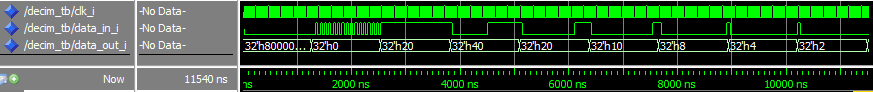
\includegraphics[width=\linewidth]{wave.png}
	\caption{Przebiegi sygnałów wejściowych i wyjściowych.}
\end{figure}

%%%%%%%%%%%%%%%%%%%%%%%%%%%%%%%%%%%%%%%%%%%%%%%%%%%%%%%%%%%%%%%%%%%%%%%%%%%%%%%

\end{document}
